In this section, we outline the basic setup, components, and architecture of feedforward neural 
networks, and describe the standard approach used for training them. While multiple types of neural 
networks exist (e.g., convolutional neural networks, recurrent neural networks), we restrict our 
attention to feedforward neural networks. All references to neural networks in this report refer 
exclusively to this type.

Throughout, we adopt the following notation: vectors are denoted using lowercase bold symbols 
(e.g., $\mathbf{x}$), while matrices are written in uppercase bold (e.g., $\mathbf{W}$). We denote 
the output of the neural network as $\hat{y}$, which approximates a target function $y$.

\subsection{Neural Networks Overview and Architecture}

A feedforward neural network defines a function \( f_\theta : \mathbb{R}^n \to \mathbb{R}^m \), 
parameterised by a collection of weight matrices and bias vectors \( \theta = \{ \mathbf{W}^{(l)},
\mathbf{b}^{(l)} \}_{l=1}^L \). It is trained to approximate a target function \( y : \mathbb{R}^n \to 
\mathbb{R}^m \) using observed or synthetically generated data.

The model takes an input vector \( \mathbf{x} \in \mathbb{R}^n \) and propagates it forward through a
sequence of $L$ layers, each composed of individual units called \emph{neurons}. 

Each \emph{neuron} in a layer performs a simple two-step operation. First, it computes a weighted
sum of its inputs and adds a bias term. Then, it applies a non-linear activation function to the result.
Specifically, if a neuron with weights \( \mathbf{w}^{(l)}_i \in \mathbb{R}^{n_{l-1}} \) and bias 
\( b^{(l)}_i \in \mathbb{R} \) receives an input vector \( \mathbf{z}^{(l-1)} \in \mathbb{R}^{n_{l-1}} \), 
then its output is given by
\[
    z^{(l)}_i = \sigma\left( (\mathbf{w}^{(l)}_i)^\top \mathbf{z}^{(l-1)} + b^{(l)}_i \right),
\]
where \( \sigma: \mathbb{R} \to \mathbb{R} \) is the neuron's fixed activation function.

A layer consists of multiple such neurons, all operating in parallel on the same input vector 
\( \mathbf{z}^{(l-1)} \), each with its own weight vector and bias. The outputs from all neurons in the
layer are collected into a vector \( \mathbf{z}^{(l)} \in \mathbb{R}^{n_l} \), where \( n_l \) denotes 
the number of neurons in layer \( l \). Letting \( \mathbf{W}^{(l)} \in 
\mathbb{R}^{n_l \times n_{l-1}} \) be the matrix whose rows are the individual neuron weight vectors 
\( (\mathbf{w}^{(l)}_i)^\top \), and \( \mathbf{b}^{(l)} \in \mathbb{R}^{n_l} \) the vector of biases, 
we can express the full layer computation compactly as
\[
    \mathbf{z}^{(l)} = \sigma\left( \mathbf{W}^{(l)} \mathbf{z}^{(l-1)} + \mathbf{b}^{(l)} \right),
\]
with the activation function \( \sigma \) now applied componentwise.

The network as a whole consists of a composition of such layers. Starting from the input 
vector \( \mathbf{z}^{(0)} = \mathbf{x} \), each successive layer transforms the output of the previous
one. For a network with \( L \) layers, the computation proceeds recursively:
\[
    \mathbf{z}^{(l)} = \sigma^{(L)}\left( \mathbf{W}^{(l)} \mathbf{z}^{(l-1)} + \mathbf{b}^{(l)} 
    \right), \quad \text{for } l = 1, \dots, L-1,
\]
with the final output given by
\[
    \hat{\mathbf{y}} = f_\theta(\mathbf{x}) = \sigma^{(l)}(\mathbf{W}^{(L)} \mathbf{z}^{(L-1)} + 
    \mathbf{b}^{(L)}).
\]

The total set of network parameters \( \theta = \{ \mathbf{W}^{(l)}, \mathbf{b}^{(l)} \}_{l=1}^L \) 
are learned during training. The architecture is defined by the number of layers \( L \), the number 
of neurons \( n_l \) in each layer, and the choice of activation functions \( \sigma^{(l)} \).
The first and last layers are termed the input and output layers respectively, while intermediate 
layers are termed hidden layers. Figure \ref{fig:nn-architecture} gives an an illustrative diagram of 
a neural network architecture, with each neuron denoted by a circle, and the lines connecting each
neuron indicating an output of a single neuron being passed as an input to subsequent neurons for 
processing.

\begin{figure}[h]
    \centering
    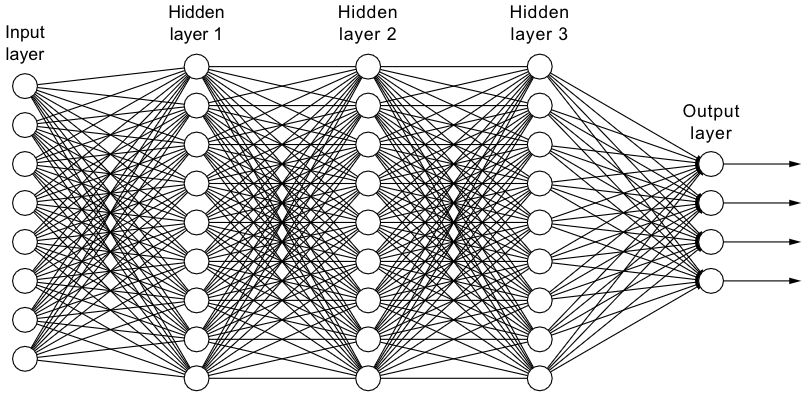
\includegraphics[width=0.7\textwidth]{graphics/neural_network_image.png}
    \caption{Illustration of a fully connected feedforward neural network with three hidden layers. 
    Each neuron computes an affine transformation of its inputs followed by a non-linear activation.}
    \label{fig:nn-architecture}
\end{figure}


Common activation functions used include:

\begin{itemize}
    \item \textbf{Hyperbolic tangent (tanh):} \quad 
    \( \sigma(x) = \tanh(x) = \dfrac{e^x - e^{-x}}{e^x + e^{-x}} \), 
    often preferred for its smoothness and differentiability.

    \item \textbf{Rectified Linear Unit (ReLU):} \quad 
    \( \sigma(x) = \max(0, x) \), 
    though not ideal when higher-order derivatives are needed.

    \item \textbf{Leaky ReLU:} \quad 
    \( \sigma(x) = 
    \begin{cases}
        x, & \text{if } x \geq 0 \\
        \alpha x, & \text{if } x < 0
    \end{cases} \), for small \( \alpha > 0 \).
    
    \item \textbf{Sinusoidal:} \quad 
    \( \sigma(x) = \sin(x) \), useful for representing oscillatory functions.
\end{itemize}

In this report we will restrict ourselves to considering these activation functions.


\subsection{Training}\label{sec:nn_training}

The parameters of a neural network — namely the weight matrices and bias vectors 
\( \theta = \{ \mathbf{W}^{(l)}, \mathbf{b}^{(l)} \}_{l=1}^L \) — are learned through a process 
called \emph{training}. The goal of training is to find a parameter set \( \theta \) such that the 
network output \( \hat{y} = f_\theta(\mathbf{x}) \) closely approximates the desired output \( y \) 
over a set of inputs \( \mathbf{x} \in \mathbb{R}^n \).

This is accomplished by defining a \emph{loss function} \( \mathcal{L}(\theta) \) that quantifies the 
discrepancy between the network predictions and the target values across a training dataset. 
In this way, training becomes a minimisation problem, where the goal is to find the parameter 
configuration $\theta^*$ that minimises the loss function $\mathcal{L}$.
When the desired outputs are continuous, a common choice is the mean squared error (MSE):
\[
    \mathcal{L}(\theta) = \frac{1}{N} \sum_{i=1}^{N} \left\| f_\theta(\mathbf{x}^{(i)}) - y^{(i)} \right\|^2,
\]
where \( \{ (\mathbf{x}^{(i)}, y^{(i)}) \}_{i=1}^N \) is the training dataset of input-output pairs.

To minimise the loss function, \( \mathcal{L}(\theta) \), a gradient-based approach 
is typically used. This requires computing the gradient of the loss with respect to all network 
parameters. This is made efficient by the \emph{backpropagation algorithm}, which systematically 
applies the chain rule of calculus to compute these derivatives by propagating error signals backward 
through the layers of the network.

Let us denote the output of layer \( l \) as \( \mathbf{z}^{(l)} \in \mathbb{R}^{n_l} \), computed via
\[
    \mathbf{z}^{(l)} = \sigma^{(l)}\left( \mathbf{a}^{(l)} \right), \quad \text{where} \quad \mathbf{a}^{(l)} = \mathbf{W}^{(l)} \mathbf{z}^{(l-1)} + \mathbf{b}^{(l)},
\]
and \( \sigma^{(l)} \) is the activation function applied componentwise.

Define the error signal at layer \( l \) as
\[
    \boldsymbol{\delta}^{(l)} := \frac{\partial \mathcal{L}}{\partial \mathbf{a}^{(l)}},
\]
which captures the sensitivity of the loss to the pre-activation input at that layer. The error at the final layer \( L \) is computed using the derivative of the loss function with respect to the network output:
\[
    \boldsymbol{\delta}^{(L)} = \nabla_{\hat{\mathbf{y}}} \mathcal{L} \odot \sigma'^{(L)}\left( \mathbf{a}^{(L)} \right),
\]
where \( \odot \) denotes elementwise (Hadamard) product and \( \sigma'^{(L)} \) is the derivative of the activation function at the final layer.

For hidden layers \( l = L-1, \dots, 1 \), the errors are computed recursively using
\[
    \boldsymbol{\delta}^{(l)} = \left( (\mathbf{W}^{(l+1)})^\top \boldsymbol{\delta}^{(l+1)} \right) \odot \sigma'^{(l)}\left( \mathbf{a}^{(l)} \right).
\]

Once the error signals are computed for each layer, the gradients of the loss with respect to the weights and biases are given by
\[
    \frac{\partial \mathcal{L}}{\partial \mathbf{W}^{(l)}} = \boldsymbol{\delta}^{(l)} (\mathbf{z}^{(l-1)})^\top, \quad
    \frac{\partial \mathcal{L}}{\partial \mathbf{b}^{(l)}} = \boldsymbol{\delta}^{(l)}.
\]

These gradients are then used in an optimisation routine (e.g., stochastic gradient descent) to update the parameters:
\[
    \mathbf{W}^{(l)} \leftarrow \mathbf{W}^{(l)} - \eta \frac{\partial \mathcal{L}}{\partial \mathbf{W}^{(l)}}, \quad
    \mathbf{b}^{(l)} \leftarrow \mathbf{b}^{(l)} - \eta \frac{\partial \mathcal{L}}{\partial \mathbf{b}^{(l)}},
\]
where \( \eta > 0 \) is the learning rate.

This process is repeated iteratively over the training data until convergence to a (local) minimum of the loss function. In practice, more advanced optimisers such as Adam or RMSProp are often used, which adaptively adjust the learning rate based on estimates of past gradients.
